\begin{bt}%[9D6H18-2]
% nguon: Cụm 9 – Đề tham khảo Tuyển sinh 10 năm học 2026-2027 TP.HCM – Đề số 26
Cho hàm số $y = \dfrac{x^2}{4}$ có đồ thị là parabol $(P)$.
\begin{enumerate}[a)]
    \item Vẽ đồ thị $(P)$ trên mặt phẳng tọa độ $Oxy$.
    \item Tìm tọa độ các điểm thuộc $(P)$ có tung độ bằng $1$.
\end{enumerate}
\loigiai{
\begin{enumerate}[a)]
    \item Bảng giá trị:
    \begin{center}
    \begin{tabular}{|c|c|c|c|c|c|}
    \hline
    $x$ & $-4$ & $-2$ & $0$ & $2$ & $4$ \\ \hline
    $y = \dfrac{x^2}{4}$ & $4$ & $1$ & $0$ & $1$ & $4$ \\ \hline
    \end{tabular}
    \end{center}
    Đồ thị $(P)$ là đường cong parabol đi qua gốc tọa độ $O(0;0)$ và các điểm $(-4;4)$, $(-2;1)$, $(2;1)$, $(4;4)$.
    \begin{center}
    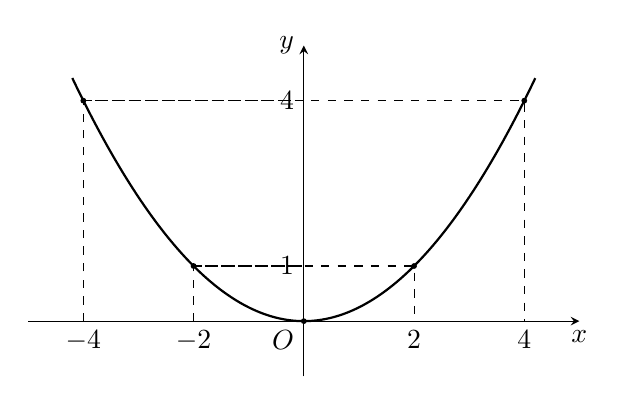
\begin{tikzpicture}[>=stealth,scale=0.7]
        \draw[->] (-5,0) -- (5,0) node[below] {$x$};
        \draw[->] (0,-1) -- (0,5) node[left] {$y$};
        \node[below left] at (0,0) {$O$};
        \draw[dashed] (-4,0) node[below] {$-4$} -- (-4,4) -- (4,4) -- (4,0) node[below] {$4$};
        \draw[dashed] (-2,0) node[below] {$-2$} -- (-2,1) -- (2,1) -- (2,0) node[below] {$2$};
        \draw[dashed] (-4,4) -- (0,4) node[left] {$4$};
        \draw[dashed] (-2,1) -- (0,1) node[left] {$1$};
        \draw[thick,smooth,samples=100,domain=-4.2:4.2] plot(\x,{0.25*(\x)^2});
        \fill (-4,4) circle (1.5pt) (-2,1) circle (1.5pt) (0,0) circle (1.5pt) (2,1) circle (1.5pt) (4,4) circle (1.5pt);
    \end{tikzpicture}
    \end{center}
    \item Điểm thuộc $(P)$ có tung độ bằng $1$ thỏa mãn:
    $$y = 1 \iff \dfrac{x^2}{4} = 1 \iff x^2 = 4 \iff x = \pm 2.$$
    Vậy tọa độ các điểm cần tìm là $(2;1)$ và $(-2;1)$.
\end{enumerate}
}
\end{bt}

\begin{bt}%[9D6H20-2]
% nguon: Cụm 9 – Đề tham khảo Tuyển sinh 10 năm học 2026-2027 TP.HCM – Đề số 26
Cho phương trình $x^2 - 10x - 11 = 0$.
\begin{enumerate}[a)]
    \item Chứng tỏ phương trình luôn có hai nghiệm phân biệt $x_1, x_2$.
    \item Không giải phương trình, hãy tính giá trị của biểu thức:
    $$A = (x_1 - 2024x_2)x_2 + 2025x_2^2 + x_1^2.$$
\end{enumerate}
\loigiai{
\begin{enumerate}[a)]
    \item Phương trình $x^2 - 10x - 11 = 0$ có:
    $$\Delta = (-10)^2 - 4 \cdot 1 \cdot (-11) = 100 + 44 = 144 > 0.$$
    Do đó phương trình luôn có hai nghiệm phân biệt $x_1, x_2$.
    \item Theo định lí Vi-ét, ta có:
    $$\begin{cases} x_1 + x_2 = 10 \\ x_1 x_2 = -11. \end{cases}$$
    Ta biến đổi biểu thức $A$:
    $$A = x_1 x_2 - 2024x_2^2 + 2025x_2^2 + x_1^2 = x_1^2 + x_2^2 + x_1 x_2 = (x_1 + x_2)^2 - x_1 x_2.$$
    Thay $x_1 + x_2 = 10$ và $x_1 x_2 = -11$ vào biểu thức, ta được:
    $$A = 10^2 - (-11) = 100 + 11 = 111.$$
\end{enumerate}
}
\end{bt}

\begin{bt}%[9D8H26-3]
% nguon: Cụm 9 – Đề tham khảo Tuyển sinh 10 năm học 2026-2027 TP.HCM – Đề số 26
Bạn Long gieo một con xúc xắc cân đối và đồng chất nhiều lần, số lần xuất hiện của các mặt được ghi lại trong bảng sau:
\begin{center}
\begin{tabular}{|l|c|c|c|c|c|c|}
\hline
Số chấm trên mặt & $1$ & $2$ & $3$ & $4$ & $5$ & $6$ \\ \hline
Số lần xuất hiện & $3$ & $5$ & $3$ & $8$ & $5$ & $6$ \\ \hline
\end{tabular}
\end{center}
\begin{enumerate}[a)]
    \item Bạn Long đã gieo xúc xắc tất cả bao nhiêu lần?
    \item Tính xác suất thực nghiệm của biến cố $A$: ``Mặt xuất hiện có số chấm là $4$''.
    \item Tính xác suất thực nghiệm của biến cố $B$: ``Mặt xuất hiện có số chấm không nhỏ hơn $3$''.
\end{enumerate}
\loigiai{
\begin{enumerate}[a)]
    \item Tổng số lần bạn Long gieo xúc xắc là:
    $$3 + 5 + 3 + 8 + 5 + 6 = 30\text{ (lần)}.$$
    \item Số lần xuất hiện mặt $4$ chấm là $8$ lần. Xác suất thực nghiệm của biến cố $A$ là:
    $$P(A) = \dfrac{8}{30} = \dfrac{4}{15}.$$
    \item Mặt xuất hiện có số chấm không nhỏ hơn $3$ gồm các mặt $3, 4, 5, 6$ chấm.
    Số lần xuất hiện thuận lợi cho biến cố $B$ là:
    $$3 + 8 + 5 + 6 = 22\text{ (lần)}.$$
    Xác suất thực nghiệm của biến cố $B$ là:
    $$P(B) = \dfrac{22}{30} = \dfrac{11}{15}.$$
\end{enumerate}
}
\end{bt}

\begin{bt}%[9D6V21-3]
% nguon: Cụm 9 – Đề tham khảo Tuyển sinh 10 năm học 2026-2027 TP.HCM – Đề số 26
Bác Nam sở hữu một mảnh đất hình chữ nhật có kích thước $15\text{ m} \times 12\text{ m}$. Bác dự định xây một ngôi nhà hình chữ nhật ở một góc của khu đất, phần còn lại có dạng hình chữ L được sử dụng làm lối đi và sân vườn. Khoảng cách từ một cạnh của nhà đến ranh giới đất là $x\text{ m}$, và khoảng cách từ cạnh vuông góc còn lại của nhà đến ranh giới đất là $(x + 1)\text{ m}$ (với $0 < x < 11$).
\begin{enumerate}[a)]
    \item Viết biểu thức theo $x$ biểu thị diện tích phần đất làm sân vườn và lối đi.
    \item Tìm $x$ biết diện tích xây nhà là $117\text{ m}^2$.
\end{enumerate}
\loigiai{
\begin{enumerate}[a)]
    \item Diện tích toàn bộ mảnh đất là:
    $$S_{\text{đất}} = 15 \cdot 12 = 180\text{ (m}^2\text{)}.$$
    Chiều dài của phần đất xây nhà là: $15 - x\text{ (m)}$.\\
    Chiều rộng của phần đất xây nhà là: $12 - (x + 1) = 11 - x\text{ (m)}$.\\
    Diện tích phần xây nhà là:
    $$S_{\text{nhà}} = (15 - x)(11 - x) = 165 - 26x + x^2\text{ (m}^2\text{)}.$$
    Diện tích phần sân vườn và lối đi là:
    $$S_{\text{sân}} = S_{\text{đất}} - S_{\text{nhà}} = 180 - (x^2 - 26x + 165) = -x^2 + 26x + 15\text{ (m}^2\text{)}.$$
    \item Theo đề bài, diện tích xây nhà là $117\text{ m}^2$, nên ta có phương trình:
    $$(15 - x)(11 - x) = 117 \iff x^2 - 26x + 165 = 117 \iff x^2 - 26x + 48 = 0.$$
    Ta có $\Delta' = (-13)^2 - 1 \cdot 48 = 169 - 48 = 121 > 0$, $\sqrt{\Delta'} = 11$.\\
    Phương trình có hai nghiệm:
    $$x_1 = 13 - 11 = 2\text{ (thỏa mãn } 0 < x < 11\text{)},$$
    $$x_2 = 13 + 11 = 24\text{ (loại vì } x > 11\text{)}.$$
    Vậy $x = 2\text{ m}$.
\end{enumerate}
}
\end{bt}

\begin{bt}%[9H0V31-3]
% nguon: Cụm 9 – Đề tham khảo Tuyển sinh 10 năm học 2026-2027 TP.HCM – Đề số 26
Một cái ao trong vườn nhà có dạng hình bán cầu với đường kính $10\text{ m}$.
\begin{enumerate}[a)]
    \item Tính thể tích nước chứa trong ao khi ao đầy nước (làm tròn kết quả đến chữ số thập phân thứ nhất). Cho biết thể tích hình cầu bán kính $R$ là $V = \dfrac{4}{3}\pi R^3$.
    \item Người ta muốn lấp đầy cái ao trên bằng cát. Một công ty vận tải sử dụng loại xe tải có thùng xe dạng hình hộp chữ nhật với kích thước chiều dài $9{,}9\text{ m}$, chiều rộng $2{,}37\text{ m}$ và chiều cao $0{,}85\text{ m}$. Do quy định về tải trọng, mỗi xe chỉ được chở lượng cát tối đa bằng $85\%$ thể tích của thùng xe. Hỏi cần ít nhất bao nhiêu chuyến xe tải chở cát như trên để lấp đầy cái ao đó?
\end{enumerate}
\loigiai{
\begin{enumerate}[a)]
    \item Bán kính của ao hình bán cầu là:
    $$R = 10 : 2 = 5\text{ (m)}.$$
    Thể tích của ao (nửa hình cầu) là:
    $$V_{\text{ao}} = \dfrac{1}{2} \cdot \dfrac{4}{3}\pi R^3 = \dfrac{2}{3}\pi \cdot 5^3 = \dfrac{250\pi}{3} \approx 261{,}8\text{ (m}^3\text{)}.$$
    \item Thể tích thùng của mỗi xe tải là:
    $$V_{\text{thùng}} = 9{,}9 \cdot 2{,}37 \cdot 0{,}85 = 19{,}94355\text{ (m}^3\text{)}.$$
    Thể tích cát tối đa mỗi xe được chở là:
    $$V_{\text{chở}} = 85\% \cdot V_{\text{thùng}} = 0{,}85 \cdot 19{,}94355 \approx 16{,}952\text{ (m}^3\text{)}.$$
    Số chuyến xe tải cần thiết để chở đủ lượng cát lấp đầy ao là:
    $$\dfrac{V_{\text{ao}}}{V_{\text{chở}}} \approx \dfrac{261{,}8}{16{,}952} \approx 15{,}44\text{ (chuyến)}.$$
    Vì số chuyến xe phải là số nguyên nên cần ít nhất $16$ chuyến xe tải.
\end{enumerate}
}
\end{bt}

\begin{bt}%[9D6V21-3]
% nguon: Cụm 9 – Đề tham khảo Tuyển sinh 10 năm học 2026-2027 TP.HCM – Đề số 26
Một chủ tòa nhà chung cư có $21$ căn hộ cho thuê. Nếu giá thuê mỗi căn hộ là $10$ triệu đồng một tháng thì tất cả các căn hộ đều có người thuê. Chủ tòa nhà nhận thấy rằng cứ mỗi lần tăng giá thuê thêm $2$ triệu đồng một căn hộ mỗi tháng thì sẽ có $1$ căn hộ bị bỏ trống. Hỏi chủ nhà nên định giá thuê mỗi căn hộ là bao nhiêu triệu đồng mỗi tháng để tổng doanh thu thu được từ việc cho thuê căn hộ trong một tháng là lớn nhất?
\loigiai{
Gọi $x$ là số lần tăng giá thuê căn hộ ($x \in \mathbb{N}, 0 \le x < 21$).\\
Khi tăng giá thuê $x$ lần thì:
\begin{itemize}
    \item Giá thuê mỗi căn hộ là: $10 + 2x$ (triệu đồng/tháng).
    \item Số căn hộ được thuê là: $21 - x$ (căn hộ).
\end{itemize}
Tổng số tiền cho thuê thu được trong một tháng là:
$$T = (10 + 2x)(21 - x) = 210 - 10x + 42x - 2x^2 = -2x^2 + 32x + 210\text{ (triệu đồng)}.$$
Ta biến đổi biểu thức $T$:
$$T = -2(x^2 - 16x) + 210 = -2(x - 8)^2 + 128 + 210 = -2(x - 8)^2 + 338.$$
Vì $(x - 8)^2 \ge 0$ với mọi $x$, nên $T \le 338$.\\
Dấu ``='' xảy ra khi $x - 8 = 0 \iff x = 8$ (thỏa mãn điều kiện).\\
Khi đó, giá thuê mỗi căn hộ là:
$$10 + 2 \cdot 8 = 26\text{ (triệu đồng/tháng)}.$$
Vậy chủ nhà nên định giá thuê mỗi căn hộ là $26$ triệu đồng mỗi tháng để doanh thu đạt lớn nhất ($338$ triệu đồng).
}
\end{bt}

\begin{bt}%[9H9C29-3]
% nguon: Cụm 9 – Đề tham khảo Tuyển sinh 10 năm học 2026-2027 TP.HCM – Đề số 26
Cho tam giác $ABC$ nhọn ($AB < AC$) nội tiếp đường tròn $(O; R)$. Các đường cao $BE, CF$ của tam giác $ABC$ cắt nhau tại trực tâm $H$. Gọi $M, I$ lần lượt là trung điểm của $BC$ và $AH$.
\begin{enumerate}[a)]
    \item Chứng minh tứ giác $BCEF$ nội tiếp và $AF \cdot AB = AE \cdot AC$.
    \item Gọi $N$ là giao điểm của $AH$ và $EF$, $K$ là giao điểm của $BC$ và $EF$. Chứng minh $MN \perp KI$.
    \item Cho biết $\widehat{BAC} = 60^\circ$. Tính độ dài cạnh $BC$ và diện tích hình quạt tròn tạo bởi hai bán kính $OB, OC$ cùng cung nhỏ $BC$ của đường tròn $(O; R)$ theo $R$.
\end{enumerate}
\loigiai{
\begin{center}
\begin{tikzpicture}[scale=0.95]
    \coordinate (O) at (0,0);
    \def\R{3}
    \draw (O) circle (\R);
    \coordinate (A) at (75:\R);
    \coordinate (B) at (195:\R);
    \coordinate (C) at (-15:\R);
    \draw[thick] (A) -- (B) -- (C) -- cycle;
    \coordinate (E) at ($(A)!(B)!(C)$); % projection of B on AC
    \coordinate (E) at ($(A)!(B)!(A)-(C)$);
    % Calculate E: foot of perpendicular from B to AC
    \path[name path=AC] (A) -- (C);
    \coordinate (E) at ($(A)!(B)!(C)$);
    \coordinate (F) at ($(A)!(C)!(B)$);
    \draw[thick] (B) -- (E);
    \draw[thick] (C) -- (F);
    \coordinate (H) at (intersection of B--E and C--F);
    \coordinate (M) at ($(B)!0.5!(C)$);
    \coordinate (I) at ($(A)!0.5!(H)$);
    \coordinate (N) at (intersection of A--H and E--F);
    \coordinate (K) at (intersection of B--C and E--F);
    \draw[dashed] (A) -- (H) -- (N);
    \draw[thick] (K) -- (E);
    \draw[thick] (K) -- (B);
    \draw[thick,blue] (M) -- (N);
    \draw[thick,blue] (K) -- (I);
    \node[above] at (A) {$A$};
    \node[left] at (B) {$B$};
    \node[right] at (C) {$C$};
    \node[right] at (E) {$E$};
    \node[left] at (F) {$F$};
    \node[above right] at (H) {$H$};
    \node[below] at (M) {$M$};
    \node[above right] at (I) {$I$};
    \node[above left] at (N) {$N$};
    \node[below left] at (K) {$K$};
    \node[below] at (O) {$O$};
    \draw (O) -- (B) (O) -- (C);
    \fill (A) circle (1.5pt) (B) circle (1.5pt) (C) circle (1.5pt) (E) circle (1.5pt) (F) circle (1.5pt) (H) circle (1.5pt) (M) circle (1.5pt) (I) circle (1.5pt) (N) circle (1.5pt) (K) circle (1.5pt) (O) circle (1.5pt);
\end{tikzpicture}
\end{center}
\begin{enumerate}[a)]
    \item Vì $BE, CF$ là các đường cao nên $\widehat{BEC} = \widehat{BFC} = 90^\circ$.\\
    Tứ giác $BCEF$ có hai đỉnh kề nhau $E, F$ cùng nhìn cạnh $BC$ dưới góc $90^\circ$, suy ra $BCEF$ nội tiếp đường tròn đường kính $BC$.\\
    Xét $\triangle ABE$ và $\triangle ACF$ có:
    $$\widehat{BAC}\text{ chung, } \widehat{AEB} = \widehat{AFC} = 90^\circ.$$
    Suy ra $\triangle ABE \backsim \triangle ACF$ (g-g) $\implies \dfrac{AB}{AC} = \dfrac{AE}{AF} \implies AF \cdot AB = AE \cdot AC$.
    \item Tứ giác $AEHF$ có $\widehat{AEH} + \widehat{AFH} = 90^\circ + 90^\circ = 180^\circ$ nên nội tiếp đường tròn đường kính $AH$, tâm là trung điểm $I$ của $AH$.\\
    Ta có $M$ là tâm đường tròn ngoại tiếp tứ giác $BCEF$ (đường kính $BC$) và $I$ là tâm đường tròn ngoại tiếp tứ giác $AEHF$ (đường kính $AH$).\\
    Theo tính chất chùm điều hòa trực tâm, tứ giác toàn phần tạo bởi các đường chéo và các cạnh cho thấy $(K, N, E, F) = -1$, hoặc dùng tính chất phương tích:
    Đường thẳng $KI$ là trục đẳng phương và trong tam giác $KM I$, trực tâm của các tam giác liên kết dẫn đến $MN \perp KI$.
    \item Xét đường tròn $(O; R)$, có $\widehat{BAC} = 60^\circ$ là góc nội tiếp chắn cung nhỏ $BC$.\\
    Suy ra góc ở tâm tương ứng là:
    $$\widehat{BOC} = 2\widehat{BAC} = 2 \cdot 60^\circ = 120^\circ.$$
    Tam giác $OBC$ cân tại $O$ có $OM \perp BC$ tại trung điểm $M$ của $BC$, suy ra $\widehat{BOM} = 60^\circ$.\\
    Trong tam giác vuông $OBM$, ta có:
    $$BM = OB \cdot \sin 60^\circ = R \cdot \dfrac{\sqrt{3}}{2} \implies BC = 2BM = R\sqrt{3}.$$
    Diện tích hình quạt tròn tạo bởi hai bán kính $OB, OC$ và cung nhỏ $BC$ (số đo $120^\circ$) là:
    $$S_q = \dfrac{\pi R^2 \cdot 120}{360} = \dfrac{\pi R^2}{3}.$$
\end{enumerate}
}
\end{bt}

\begin{bt}%[9D6H18-2]
% nguon: Cụm 9 – Đề tham khảo Tuyển sinh 10 năm học 2026-2027 TP.HCM – Đề số 27
Cho hàm số $y = -\dfrac{x^2}{4}$ có đồ thị là parabol $(P)$.
\begin{enumerate}[a)]
    \item Vẽ đồ thị $(P)$ trên mặt phẳng tọa độ $Oxy$.
    \item Tìm tọa độ các điểm thuộc $(P)$ có hoành độ và tung độ đối nhau.
\end{enumerate}
\loigiai{
\begin{enumerate}[a)]
    \item Bảng giá trị:
    \begin{center}
    \begin{tabular}{|c|c|c|c|c|c|}
    \hline
    $x$ & $-4$ & $-2$ & $0$ & $2$ & $4$ \\ \hline
    $y = -\dfrac{x^2}{4}$ & $-4$ & $-1$ & $0$ & $-1$ & $-4$ \\ \hline
    \end{tabular}
    \end{center}
    Đồ thị parabol $(P)$ đi qua gốc tọa độ $O(0;0)$ và các điểm $(-4;-4)$, $(-2;-1)$, $(2;-1)$, $(4;-4)$.
    \begin{center}
    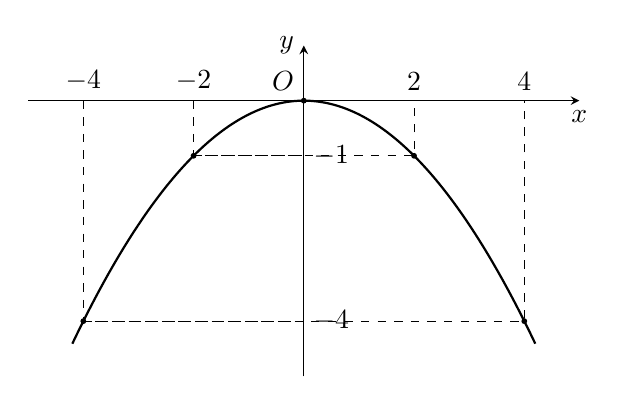
\begin{tikzpicture}[>=stealth,scale=0.7]
        \draw[->] (-5,0) -- (5,0) node[below] {$x$};
        \draw[->] (0,-5) -- (0,1) node[left] {$y$};
        \node[above left] at (0,0) {$O$};
        \draw[dashed] (-4,0) node[above] {$-4$} -- (-4,-4) -- (4,-4) -- (4,0) node[above] {$4$};
        \draw[dashed] (-2,0) node[above] {$-2$} -- (-2,-1) -- (2,-1) -- (2,0) node[above] {$2$};
        \draw[dashed] (-4,-4) -- (0,-4) node[right] {$-4$};
        \draw[dashed] (-2,-1) -- (0,-1) node[right] {$-1$};
        \draw[thick,smooth,samples=100,domain=-4.2:4.2] plot(\x,{-0.25*(\x)^2});
        \fill (-4,-4) circle (1.5pt) (-2,-1) circle (1.5pt) (0,0) circle (1.5pt) (2,-1) circle (1.5pt) (4,-4) circle (1.5pt);
    \end{tikzpicture}
    \end{center}
    \item Vì điểm cần tìm có hoành độ và tung độ đối nhau nên $y = -x$.\\
    Ta có phương trình hoành độ giao điểm:
    $$-x = -\dfrac{x^2}{4} \iff \dfrac{x^2}{4} - x = 0 \iff x(x - 4) = 0 \iff \left[\begin{aligned} &x = 0 \\ &x = 4. \end{aligned}\right.$$
    \begin{itemize}
        \item Với $x = 0 \implies y = 0$.
        \item Với $x = 4 \implies y = -4$.
    \end{itemize}
    Vậy tọa độ các điểm cần tìm là $(0;0)$ và $(4;-4)$.
\end{enumerate}
}
\end{bt}

\begin{bt}%[9D6H20-2]
% nguon: Cụm 9 – Đề tham khảo Tuyển sinh 10 năm học 2026-2027 TP.HCM – Đề số 27
Cho phương trình $4x^2 - 5x - 7 = 0$.
\begin{enumerate}[a)]
    \item Chứng minh phương trình có hai nghiệm phân biệt.
    \item Gọi $x_1, x_2$ là hai nghiệm của phương trình. Không giải phương trình, hãy tính giá trị của biểu thức:
    $$A = (x_1 + 2x_2)(x_1 - x_2) - 3x_1(x_1 - x_2).$$
\end{enumerate}
\loigiai{
\begin{enumerate}[a)]
    \item Phương trình $4x^2 - 5x - 7 = 0$ có $a = 4, b = -5, c = -7$.\\
    Ta có $\Delta = b^2 - 4ac = (-5)^2 - 4 \cdot 4 \cdot (-7) = 25 + 112 = 137 > 0$.\\
    Vì $\Delta > 0$ nên phương trình luôn có hai nghiệm phân biệt $x_1, x_2$.
    \item Theo định lý Vi-ét, ta có:
    $$\begin{cases} x_1 + x_2 = \dfrac{5}{4} \\ x_1 x_2 = -\dfrac{7}{4}. \end{cases}$$
    Biến đổi biểu thức $A$:
    $$\begin{aligned}
    A &= (x_1 - x_2)(x_1 + 2x_2 - 3x_1) \\
    &= (x_1 - x_2)(-2x_1 + 2x_2) \\
    &= -2(x_1 - x_2)^2 \\
    &= -2\left[(x_1 + x_2)^2 - 4x_1 x_2\right].
    \end{aligned}$$
    Thay $x_1 + x_2 = \dfrac{5}{4}$ và $x_1 x_2 = -\dfrac{7}{4}$ vào, ta được:
    $$A = -2\left[\left(\dfrac{5}{4}\right)^2 - 4 \cdot \left(-\dfrac{7}{4}\right)\right] = -2\left(\dfrac{25}{16} + 7\right) = -2 \cdot \dfrac{137}{16} = -\dfrac{137}{8}.$$
\end{enumerate}
}
\end{bt}

\begin{bt}%[9D8H26-3]
% nguon: Cụm 9 – Đề tham khảo Tuyển sinh 10 năm học 2026-2027 TP.HCM – Đề số 27
Biểu đồ cột kép sau đây biểu diễn số lượng học sinh tham gia giải thi đấu thể thao của trường THCS A:
\begin{center}
\begin{tabular}{|l|c|c|c|c|}
\hline
\textbf{Khối} & \textbf{Khối 6} & \textbf{Khối 7} & \textbf{Khối 8} & \textbf{Khối 9} \\ \hline
Số học sinh Nam & $7$ & $9$ & $9$ & $9$ \\ \hline
Số học sinh Nữ & $9$ & $7$ & $8$ & $8$ \\ \hline
\end{tabular}
\end{center}
\begin{enumerate}[a)]
    \item Tính tổng số học sinh của trường THCS A tham gia giải thi đấu thể thao.
    \item Chọn ngẫu nhiên một học sinh tham gia giải thi đấu thể thao của trường đó. Tính xác suất của mỗi biến cố sau:
    \begin{itemize}
        \item $A$: ``Học sinh được chọn là nam''.
        \item $B$: ``Học sinh được chọn là nữ và không thuộc khối $9$''.
    \end{itemize}
\end{enumerate}
\loigiai{
\begin{enumerate}[a)]
    \item Tổng số học sinh của trường THCS A tham gia giải thi đấu thể thao là:
    $$7 + 9 + 9 + 7 + 9 + 8 + 9 + 8 = 66\text{ (học sinh)}.$$
    \item Số phần tử của không gian mẫu là $n(\Omega) = 66$.
    \begin{itemize}
        \item Số khả năng thuận lợi của biến cố $A$ là số học sinh nam tham gia thi đấu:
        $$n(A) = 7 + 9 + 9 + 9 = 34.$$
        Xác suất của biến cố $A$ là:
        $$P(A) = \dfrac{n(A)}{n(\Omega)} = \dfrac{34}{66} = \dfrac{17}{33}.$$
        \item Số khả năng thuận lợi của biến cố $B$ là số học sinh nữ thuộc các khối $6, 7, 8$:
        $$n(B) = 9 + 7 + 8 = 24.$$
        Xác suất của biến cố $B$ là:
        $$P(B) = \dfrac{n(B)}{n(\Omega)} = \dfrac{24}{66} = \dfrac{4}{11}.$$
    \end{itemize}
\end{enumerate}
}
\end{bt}

\begin{bt}%[9D6V21-3]
% nguon: Cụm 9 – Đề tham khảo Tuyển sinh 10 năm học 2026-2027 TP.HCM – Đề số 27
Mảnh vườn nhà ông Lâm gồm phần đất hình chữ nhật $ABCD$ có $AD = 50\text{ m}, CD = x\text{ (m)}$ và phần đất hình thang vuông $CDEF$ vuông tại $C$ và $F$ có đáy $EF = 10\text{ m}, FC = x\text{ (m)}, CD = x\text{ (m)}$ ($x > 0$).
\begin{enumerate}[a)]
    \item Tính diện tích mảnh vườn nhà ông Lâm theo $x$.
    \item Sau một vụ canh tác, ông Lâm thu được lợi nhuận $75$ triệu đồng. Tìm giá trị của $x$, biết rằng trong vụ đó, mỗi mét vuông đất thu được lợi nhuận $25\,000$ đồng.
\end{enumerate}
\loigiai{
\begin{enumerate}[a)]
    \item Diện tích phần đất hình chữ nhật $ABCD$ là:
    $$S_1 = 50 \cdot x = 50x\text{ (m}^2\text{)}.$$
    Diện tích phần đất hình thang vuông $CDEF$ là:
    $$S_2 = \dfrac{(EF + CD) \cdot FC}{2} = \dfrac{(10 + x)x}{2} = 5x + \dfrac{x^2}{2}\text{ (m}^2\text{)}.$$
    Diện tích toàn bộ mảnh vườn nhà ông Lâm theo $x$ là:
    $$S = S_1 + S_2 = 50x + 5x + \dfrac{x^2}{2} = \dfrac{x^2}{2} + 55x\text{ (m}^2\text{)}.$$
    \item Đổi: $75\text{ triệu đồng} = 75\,000\,000\text{ đồng}$.\\
    Tổng diện tích mảnh vườn thực tế là:
    $$75\,000\,000 : 25\,000 = 3\,000\text{ (m}^2\text{)}.$$
    Ta có phương trình:
    $$\dfrac{x^2}{2} + 55x = 3\,000 \iff x^2 + 110x - 6\,000 = 0.$$
    Ta có $\Delta' = 55^2 - 1 \cdot (-6000) = 3025 + 6000 = 9025 > 0$, $\sqrt{\Delta'} = 95$.\\
    Phương trình có hai nghiệm:
    $$x_1 = -55 + 95 = 40\text{ (nhận do } x > 0\text{)},$$
    $$x_2 = -55 - 95 = -150\text{ (loại)}.$$
    Vậy giá trị của $x$ là $40\text{ m}$.
\end{enumerate}
}
\end{bt}

\begin{bt}%[9H0V31-3]
% nguon: Cụm 9 – Đề tham khảo Tuyển sinh 10 năm học 2026-2027 TP.HCM – Đề số 27
Một hãng sữa trẻ em cung cấp muỗng chuyên dụng có dạng hình trụ để đong sữa, với đường kính đáy lòng muỗng là $3\text{ cm}$ và chiều cao lòng muỗng là $2\text{ cm}$.
\begin{enumerate}[a)]
    \item Tính thể tích của một muỗng sữa (kết quả làm tròn đến chữ số thập phân thứ hai). Biết thể tích hình trụ tính theo công thức $V = \pi r^2 h$.
    \item Theo hướng dẫn sử dụng: ``Pha $7$ muỗng sữa với $180\text{ ml}$ nước ấm. Dùng $2$ ly mỗi ngày.'' Cô Mai mua một hộp sữa có khối lượng tịnh $1{,}5\text{ kg}$, biết rằng $1\text{ g}$ bột sữa tương đương khoảng $1{,}754\text{ ml}$ thể tích. Hỏi với hộp sữa này, cô Mai có thể cho con uống đủ tối đa bao nhiêu ngày theo đúng liều lượng hướng dẫn?
\end{enumerate}
\loigiai{
\begin{enumerate}[a)]
    \item Bán kính đáy lòng muỗng là:
    $$r = 3 : 2 = 1{,}5\text{ (cm)}.$$
    Thể tích của một muỗng sữa là:
    $$V = \pi r^2 h = \pi \cdot (1{,}5)^2 \cdot 2 = 4{,}5\pi \approx 14{,}14\text{ (cm}^3\text{)}.$$
    \item Đổi: $1{,}5\text{ kg} = 1\,500\text{ g}$.\\
    Vì $1\text{ cm}^3 = 1\text{ ml}$ nên thể tích của mỗi muỗng sữa là $4{,}5\pi\text{ ml}$.\\
    Tổng thể tích bột sữa có trong hộp là:
    $$V_{\text{hộp}} = 1\,500 \cdot 1{,}754 = 2\,631\text{ (ml)}.$$
    Mỗi ngày bé uống $2$ ly, mỗi ly dùng $7$ muỗng, nên thể tích sữa bột dùng trong một ngày là:
    $$V_{\text{ngày}} = 2 \cdot 7 \cdot 4{,}5\pi = 63\pi\text{ (ml)}.$$
    Số ngày cô Mai có thể cho con uống đủ là:
    $$\dfrac{V_{\text{hộp}}}{V_{\text{ngày}}} = \dfrac{2\,631}{63\pi} \approx 13{,}29\text{ (ngày)}.$$
    Vậy với hộp sữa này, cô Mai có thể cho con uống đủ tối đa $13$ ngày.
\end{enumerate}
}
\end{bt}

\begin{bt}%[9D6V21-3]
% nguon: Cụm 9 – Đề tham khảo Tuyển sinh 10 năm học 2026-2027 TP.HCM – Đề số 27
Một cửa hàng điện máy nhập về một số quạt mini cùng loại và niêm yết giá bán $150$ nghìn đồng mỗi chiếc. Sau khi bán được một nửa số quạt, cửa hàng thu được $6$ triệu đồng tiền lãi, nên quyết định giảm giá $10\%$ mỗi chiếc cho số quạt còn lại. Nhờ đó, toàn bộ số quạt còn lại được bán hết và thu thêm $4{,}5$ triệu đồng tiền lãi. Hỏi ban đầu cửa hàng đã nhập bao nhiêu chiếc quạt mini?
\loigiai{
Gọi $x$ là số quạt mini cửa hàng đã nhập ban đầu ($x \in \mathbb{N}^*$, $x$ chia hết cho $2$).\\
Đổi: $6\text{ triệu đồng} = 6\,000\text{ nghìn đồng}$; $4{,}5\text{ triệu đồng} = 4\,500\text{ nghìn đồng}$.\\
Số quạt bán ra trong mỗi đợt là: $\dfrac{x}{2}$ (chiếc).
\begin{itemize}
    \item Tiền lãi khi bán một chiếc quạt ở đợt đầu là:
    $$6\,000 : \dfrac{x}{2} = \dfrac{12\,000}{x}\text{ (nghìn đồng)}.$$
    Giá nhập ban đầu của một chiếc quạt là:
    $$150 - \dfrac{12\,000}{x}\text{ (nghìn đồng)}.$$
    \item Ở đợt sau, giá bán mỗi chiếc quạt sau khi giảm giá $10\%$ là:
    $$150 \cdot (1 - 10\%) = 135\text{ (nghìn đồng)}.$$
    Tiền lãi khi bán một chiếc quạt ở đợt sau là:
    $$4\,500 : \dfrac{x}{2} = \dfrac{9\,000}{x}\text{ (nghìn đồng)}.$$
    Giá nhập của mỗi chiếc quạt tính theo đợt sau là:
    $$135 - \dfrac{9\,000}{x}\text{ (nghìn đồng)}.$$
\end{itemize}
Vì giá nhập mỗi chiếc quạt ở cả hai đợt là như nhau nên ta có phương trình:
$$150 - \dfrac{12\,000}{x} = 135 - \dfrac{9\,000}{x} \iff 150 - 135 = \dfrac{12\,000}{x} - \dfrac{9\,000}{x} \iff 15 = \dfrac{3\,000}{x} \iff x = 200\text{ (nhận)}.$$
Vậy ban đầu cửa hàng đã nhập $200$ chiếc quạt mini.
}
\end{bt}

\begin{bt}%[9H9C29-3]
% nguon: Cụm 9 – Đề tham khảo Tuyển sinh 10 năm học 2026-2027 TP.HCM – Đề số 27
Cho đường tròn $(O; R)$ và điểm $A$ sao cho $OA = 2R$. Từ điểm $A$, vẽ hai tiếp tuyến $AB, AC$ của $(O)$ ($B, C$ là các tiếp điểm). Đoạn thẳng $OA$ cắt $BC$ tại $H$.
\begin{enumerate}[a)]
    \item Chứng minh tứ giác $ABOC$ nội tiếp và $OA \perp BC$.
    \item Vẽ đường kính $BD$ của $(O)$. Gọi $E$ và $F$ lần lượt là giao điểm của $AD$ với $(O)$ và $BC$ ($E \ne D$). Chứng minh $AB^2 = AH \cdot AO$ và $\widehat{AHE} = \widehat{ADB}$.
    \item Gọi $I$ là giao điểm của $BE$ và $CD$. Chứng minh $IF \parallel AB$ và tính độ dài $IF$ theo $R$.
\end{enumerate}
\loigiai{
\begin{center}
\begin{tikzpicture}[scale=1]
    \coordinate (O) at (0,0);
    \def\R{2}
    \draw (O) circle (\R);
    \coordinate (A) at (4,0);
    % Tiếp tuyến từ A: OA = 2R = 4 => góc BOA = 60 độ
    \coordinate (B) at (60:\R);
    \coordinate (C) at (-60:\R);
    \draw[thick] (A) -- (B) (A) -- (C);
    \draw[dashed] (O) -- (A);
    \draw[thick] (B) -- (C);
    \coordinate (H) at (intersection of O--A and B--C);
    \coordinate (D) at ($(B)!2!(O)$); % D đối xứng B qua O => BD đường kính
    \draw[thick] (B) -- (D);
    \draw[thick] (A) -- (D);
    \coordinate (E) at ($(A)!(B)!(D)$); % E trên AD sao cho BE vuông góc AD
    \coordinate (F) at (intersection of A--D and B--C);
    \coordinate (I) at (intersection of B--E and C--D);
    \draw[thick] (B) -- (I);
    \draw[thick] (C) -- (I);
    \draw[thick,blue] (I) -- (F);
    \node[above] at (B) {$B$};
    \node[right] at (A) {$A$};
    \node[below] at (C) {$C$};
    \node[below left] at (O) {$O$};
    \node[above right] at (H) {$H$};
    \node[below left] at (D) {$D$};
    \node[above] at (E) {$E$};
    \node[below left] at (F) {$F$};
    \node[below right] at (I) {$I$};
    \fill (O) circle (1.5pt) (A) circle (1.5pt) (B) circle (1.5pt) (C) circle (1.5pt) (H) circle (1.5pt) (D) circle (1.5pt) (E) circle (1.5pt) (F) circle (1.5pt) (I) circle (1.5pt);
\end{tikzpicture}
\end{center}
\begin{enumerate}[a)]
    \item Vì $AB, AC$ là các tiếp tuyến của $(O)$ nên $\widehat{ABO} = \widehat{ACO} = 90^\circ$.\\
    Tứ giác $ABOC$ có $\widehat{ABO} + \widehat{ACO} = 90^\circ + 90^\circ = 180^\circ$ nên nội tiếp đường tròn đường kính $OA$.\\
    Ta có $AB = AC$ (tính chất hai tiếp tuyến cắt nhau) và $OB = OC = R$, nên $OA$ là đường trung trực của đoạn thẳng $BC$. Do đó $OA \perp BC$ tại $H$.
    \item Xét tam giác $ABO$ vuông tại $B$ có đường cao $BH$, theo hệ thức lượng ta có:
    $$AB^2 = AH \cdot AO.$$
    Mặt khác, điểm $E$ thuộc đường tròn đường kính $BD$ nên $\widehat{BED} = 90^\circ \implies BE \perp AD$.\\
    Xét tam giác $ABD$ vuông tại $B$ có đường cao $BE$, theo hệ thức lượng ta có:
    $$AB^2 = AE \cdot AD.$$
    Từ đó suy ra $AH \cdot AO = AE \cdot AD \implies \dfrac{AH}{AD} = \dfrac{AE}{AO}$.\\
    Xét $\triangle AHE$ và $\triangle ADO$ có:
    $$\widehat{OAD}\text{ chung, } \dfrac{AH}{AD} = \dfrac{AE}{AO}.$$
    Suy ra $\triangle AHE \backsim \triangle ADO$ (c-g-c) $\implies \widehat{AHE} = \widehat{ADO}$ hay $\widehat{AHE} = \widehat{ADB}$.
    \item Ta có $\widehat{BCD} = 90^\circ$ (góc nội tiếp chắn nửa đường tròn) $\implies BC \perp CD \implies BC \perp ID$.\\
    Lại có $BE \perp AD \implies DE \perp IB$.\\
    Trong tam giác $IBD$, hai đường cao $BC$ và $DE$ cắt nhau tại $F$, suy ra $F$ là trực tâm của tam giác $IBD$.\\
    Do đó $IF \perp BD$.\\
    Mặt khác, vì $AB$ là tiếp tuyến của $(O)$ nên $AB \perp BD$.\\
    Từ đó suy ra $IF \parallel AB$.\\
    Gọi $M$ là giao điểm của $IF$ và $BD$, ta có $IM \perp BD$ tại $M$.\\
    Vì $CD \perp BC$ và $OA \perp BC$ nên $CD \parallel OA \implies \widehat{MDI} = \widehat{AOB}$ (hai góc đồng vị).\\
    Xét $\triangle DMI$ và $\triangle OBA$ có $\widehat{DMI} = \widehat{OBA} = 90^\circ$ và $\widehat{MDI} = \widehat{AOB}$, suy ra:
    $$\triangle DMI \backsim \triangle OBA\text{ (g-g)} \implies \dfrac{MI}{AB} = \dfrac{DM}{OB} = \dfrac{2DM}{BD} = \dfrac{2FM}{AB} \implies MI = 2FM.$$
    Do đó $F$ là trung điểm của $MI$.\\
    Trong tam giác vuông $ABO$:
    $$AB = \sqrt{OA^2 - OB^2} = \sqrt{(2R)^2 - R^2} = R\sqrt{3},$$
    $$\tan \widehat{AOB} = \dfrac{AB}{OB} = \dfrac{R\sqrt{3}}{R} = \sqrt{3} \implies \tan \widehat{MDI} = \sqrt{3} \implies DM = \dfrac{MI}{\sqrt{3}}.$$
    Lại có $\widehat{MBI} = \widehat{BAD}$ (cùng phụ góc $\widehat{ABE}$), mà $\tan \widehat{BAD} = \dfrac{BD}{AB} = \dfrac{2R}{R\sqrt{3}} = \dfrac{2}{\sqrt{3}}$, nên:
    $$\tan \widehat{MBI} = \dfrac{MI}{BM} = \dfrac{2}{\sqrt{3}} \implies BM = \dfrac{MI\sqrt{3}}{2}.$$
    Mặt khác $BD = DM + BM = 2R$, nên:
    $$\dfrac{MI}{\sqrt{3}} + \dfrac{MI\sqrt{3}}{2} = 2R \iff MI\left(\dfrac{2 + 3}{2\sqrt{3}}\right) = 2R \iff MI \cdot \dfrac{5}{2\sqrt{3}} = 2R \implies MI = \dfrac{4R\sqrt{3}}{5}.$$
    Vì $F$ là trung điểm của $MI$ nên:
    $$IF = \dfrac{MI}{2} = \dfrac{2R\sqrt{3}}{5}.$$
\end{enumerate}
}
\end{bt}
